\section{Historical Development of the Abhidhamma}

\begin{figure}[h]
\centering
\input{./Diagrams/Timeline.pdf_tex}
\caption{Timeline showing key events in the development of the Abhidhamma. In my opinion, the Abhidhamma probably started to take its current form in the period between the 2\textsuperscript{nd} council (about 2400 years ago) and the 3\textsuperscript{rd} council (about 2250 years ago).}
\label{fig:Timeline}
\end{figure}

Welcome to the second lesson of this Practical Abhidhamma Course. In this lesson, we'll discuss the historical development of the Abhidhamma.

When we listen to a Dhamma talk or read a Dhamma book, we are often given information from four historical periods. The oldest source of information is the Suttas and Vinaya. These generally date to about 2500 years ago. The next oldest source, almost as old as the Suttas and Vinaya, is the Abhidhamma. The Abhidhamma was more or less complete about 2250 years ago. The Commentaries are the third source; they were compiled about 1000 to 1500 years ago. Modern writers are the fourth source. 

Each of these four sources (Suttas and Vinaya, Abhidhamma, Commentaries and modern writers) has a distinctive flavour that is a result of the historical time period when it was developed. For example, the Suttas were an oral tradition and are characterized by simple sentence structure, lots of repetition, stock descriptions and numerical lists. 

Each of these four sources build on what came earlier. Even the Suttas build on the beliefs prevalent at the time of the Buddha. For example, in the Suttas, the Buddha criticized the caste system and the doctrines of other teachers. 

When I give Dhamma talks, it is important to me that my audience is aware of my sources of information. In my talks I will say, “The Buddha said...” or “In the Abhidhamma...”\footnote{“In the Abhidhamma” means in the Abhidhamma \textit{Piṭaka}; the Abhidhammattha Sangaha is a Commentary.} or “In the Commentary...” or “In my opinion...”\footnote{I have tried to follow the same practice in this Practical Abhidhamma Course.} This contextual information allows my audience to differentiate between the core teachings of the Buddha and later additions. Later additions can be very useful, but they should be understood as being later additions.

\pagebreak

We will look at the historical development of the Abhidhamma from two perspectives; first based on the traditional accounts from the Commentaries, and then based on the current thinking of scholars. Scholars consider the traditional accounts from the Commentaries to include a mixture of fact and legend. Some of these traditional accounts may have been added by reciters to make the material more interesting to listeners.\footnote{Background stories to the Dhammapada: \url{http://www.tipitaka.net/tipitaka/dhp/index.php}}

\subsection*{Traditional account from the Commentaries}

Let’s start with the traditional account of the Abhidhamma from the Commentaries. 

According to the Commentaries,\footnote{“The Expositor” (\textit{Atthasālinī}), pages 16--18.} during the first week after gaining enlightenment, the Buddha sat under the Bodhi tree enjoying the bliss of \textit{Nibbāna}. During the second week, he stared at the Bodhi tree for one week without blinking, as a mark of respect. During the third week, he practised walking meditation. During the fourth week after enlightenment, the Buddha envisioned the Abhidhamma. He started by reflecting on the first book and went through each book in sequence. 

When the Buddha came to the fifth book, he reflected only upon the table of contents and on the list of controversies he knew would arise in about 250 years when it would be time to write this book.\footnote{According to the Dīpavaṃsa, page 119, the Third Council was 218 years after the Buddha's \textit{parinibbāna}.}

When the Buddha reached the seventh book of the Abhidhamma, Conditional Relations, he had finally found a topic worthy of his great intellect and he began emitting rays of blue, yellow, red, white, orange and dazzling light. 

In 1885, a Buddhist flag\footnote{\url{http://en.wikipedia.org/wiki/Buddhist_flag}} was designed using these colours; it was accepted as the international Buddhist flag for all schools of Buddhism in 1952. So when you see the multi-coloured Buddhist flag, think about its inspiration, the Buddha reflecting on the Abhidhamma!

\begin{figure}[H]
\begin{tabular*}{\textwidth}{L{\dimexpr0.45\textwidth-2\tabcolsep} L{\dimexpr0.55\textwidth-2\tabcolsep}}


\includegraphics[width=1\linewidth]{./Diagrams/Flag} & \tablesubheader{Blue}: Loving kindness, peace and universal compassion.\newline
\tablesubheader{Yellow}: The Middle Path – avoiding extremes, emptiness.\newline
\tablesubheader{Red}: The blessings of practice – achievement, wisdom, virtue, fortune and dignity.\newline
\tablesubheader{White}: The purity of the Dhamma – leading to liberation, outside of time or space.\newline
\tablesubheader{Orange}: The Buddha’s teachings – wisdom.\newline
\tablesubheader{Dazzling}: The combination of all the colours.\\

\end{tabular*}

\caption{According to the commentary to the Abhidhamma, blue emanated from the Buddha’s hair and eyes; Yellow from the Buddha’s skin and eyes; Red from the Buddha’s flesh, blood and eyes; White from the Buddha’s bones, teeth and eyes; Orange and dazzling emanated from different parts of the Buddha’s body.}
\label{fig:Flag}
\end{figure}

\pagebreak

\begin{figure}[h]
\centering
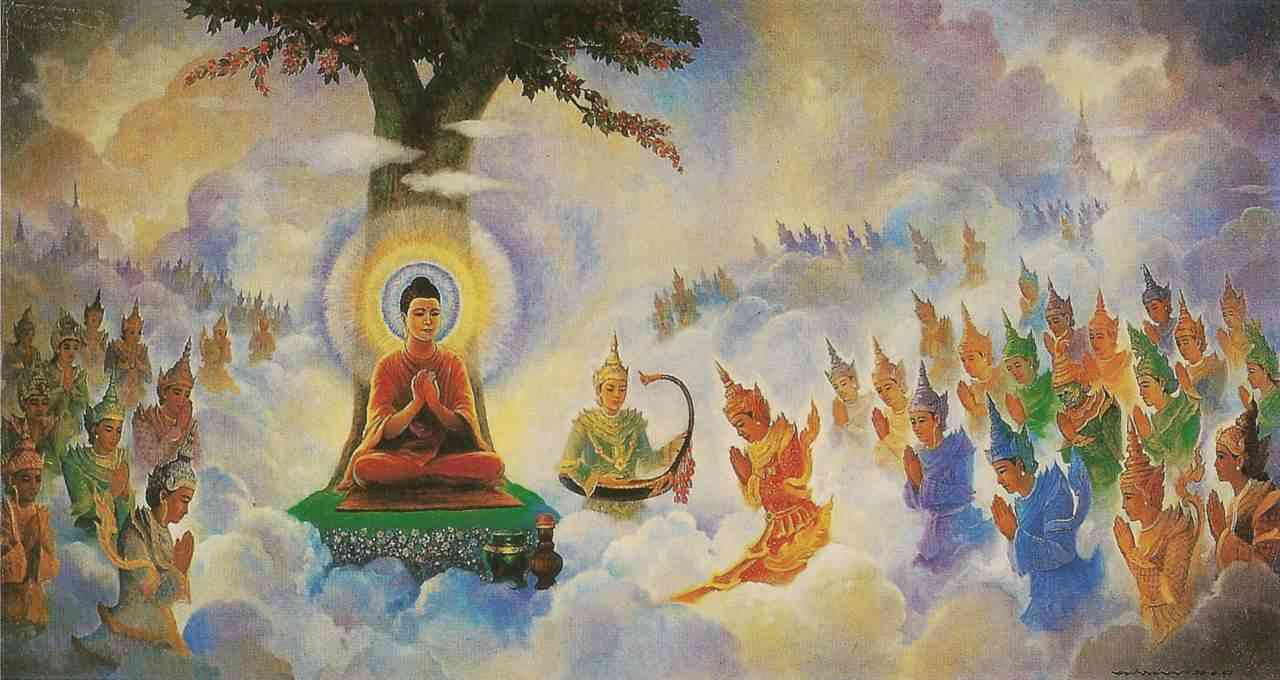
\includegraphics[width=0.9\linewidth]{./Diagrams/Tavatimsa}
\caption{Burmese depiction of the Buddha teaching Abhidhamma in Tāvatiṃsa heaven.}
\label{fig:Tavatimsa}
\end{figure}

In the seventh year after his enlightenment, the Buddha spent three months teaching Abhidhamma.\footnote{During the \textit{vassa} period (rainy season) when monks are not allowed to travel.} To teach the entire Abhidhamma, the Buddha spoke continuously, 24 hours a day, for three months.\footnote{Story in the Commentary: \url{http://www.tipitaka.net/tipitaka/dhp/verseload.php?verse=181}} No human audience could listen to such a long talk, so the Buddha taught Abhidhamma in one of the heavens,\footnote{In \textit{Tāvatiṃsa} heaven; three months in the human realm is equivalent to less than four minutes in \textit{Tāvatiṃsa} heaven. One day in \textit{Tāvatiṃsa} heaven is equivalent to 100 years of human time (See the story from the Commentary: \url{http://www.tipitaka.net/tipitaka/dhp/verseload.php?verse=048}).} as had many of the previous Buddhas.\footnote{The Buddhavamsa (\url{http://en.wikipedia.org/wiki/Buddhavamsa}) lists names of the 27 Buddhas preceding Gotama and gives a brief biography for 24 of these Buddhas. All of these 24 Buddhas started their ministry with the Dhammacakkappavattana Sutta (SN 56.11: \url{http://www.accesstoinsight.org/tipitaka/sn/sn56/sn56.011.harv.html}), but only 9 of these 24 Buddhas went to \textit{Tāvatiṃsa} heaven to preach the Abhidhamma.} He delivered this lecture to many celestial beings including his mother, who had died shortly after the Buddha was born. Each day the Buddha came down to earth to collect food. While on earth, he left a “hologram” of himself in heaven to continue teaching. Each day when he visited earth, the Buddha met with Sāriputta and said, “In the past 24 hours, I covered the following topics...” With his great wisdom, Sāriputta was able to fill in the gaps and structured the Abhidhamma texts as we have them today. Sāriputta then taught the Abhidhamma to his 500 students.\footnote{At the time of a previous Buddha, Sāriputta’s 500 students had been bats who lived together in a cave. Monks recited the Abhidhamma in this cave and the bats enjoyed the sound. The monks were therefore quick to appreciate the Abhidhamma when they heard it again from Sāriputta.}

So there are three versions of the Abhidhamma: the complete version that the Buddha taught to the celestial beings, the short summary version that the Buddha passed along to Sāriputta, and the medium-length version compiled by Sāriputta that we have today. 

According to the Commentary, the Abhidhamma was recited by Ānanda at the First Council,\footnote{\url{http://en.wikipedia.org/wiki/First_Buddhist_council}} and the fifth book, which contrasts the orthodox Theravāda view with views of other Buddhist schools, was added at the Third Council.\footnote{\url{http://en.wikipedia.org/wiki/Third_Buddhist_council}}

\subsection*{According to scholars}

Now let us consider the view of scholars. 

The word “Abhidhamma” does occur a few times in the Suttas, but not in a way that suggests it is referencing a set of texts. For example, a forest-dwelling monk is instructed to “apply himself to the higher Dhamma (Abhidhamma) and the higher discipline (Abhivinaya).”\footnote{MN 69: \url{http://awake.kiev.ua/dhamma/tipitaka/2Sutta-Pitaka/2Majjhima-Nikaya/Majjhima2/069-gulissani-e1.html}} Since the word “Abhidhamma” is paired with “Abhivinaya” and since there is no text called “Abhivinaya,” it is unlikely that in this context the word “Abhidhamma” refers to a set of texts. In addition, this Sutta focuses on the practice of a forest-dwelling monk, not a scholastic monk based in a monastery. My interpretation of this Sutta is that the forest-dwelling monk should reflect on the “essence of the Dhamma” and the “essence of the Vinaya” when alone in the forest.

The Suttas list nine ways of presenting the Dhamma, and this list does not include the Abhidhamma.\footnote{MN 22: \url{http://www.accesstoinsight.org/tipitaka/mn/mn.022.than.html\#watersnake}\\The nine ways of presenting the Dhamma: dialogues (\textit{sutta}), narratives of mixed prose and verse (\textit{geyya}), explanations (\textit{veyyakaraṇa}), verses (\textit{gāthā}), spontaneous exclamations (\textit{udāna}), quotations (\textit{itivuttaka}), birth stories (\textit{jātaka}), amazing events (\textit{abbhutadhamma}), question and answer sessions (\textit{vedalla}).} Though there may have been no collection of texts\footnote{There were no written texts at the time of the Buddha; just different types of “memorized collections.”} called Abhidhamma during the time of the Buddha, there were many Suttas in which the Buddha analyzed things using methods from the Abhidhamma. For example, the Buddha defined “the all” as “eye and \textbf{Visible-forms}, ear and \textbf{Sounds}, nose and \textbf{Odours}, tongue and \textbf{Tastes}, body and tactile objects, intellect and ideas,”\footnote{SN 35.23: \url{http://www.accesstoinsight.org/tipitaka/sn/sn35/sn35.023.than.html}; the Pāḷi terms translated as “intellect” and “ideas” are “\textit{mano}” and “\textit{dhammā}” (\textit{dhammā} is the plural of \textit{dhamma}).} saying nothing was excluded from this list.

Shortly before his \textit{parinibbāna}, the Buddha was asked who would be his successor. The Buddha replied, “Be islands unto yourselves, refuges unto yourselves, seeking no external refuge; with the Dhamma as your island, the Dhamma as your refuge, seeking no other refuge.”\footnote{DN 16: \url{http://www.accesstoinsight.org/tipitaka/dn/dn.16.1-6.vaji.html\#island}}

If the Dhamma was to be the guide, it needed to be clear, and the Suttas sometimes give apparently conflicting information. For example in one Sutta, an argument broke out between two of the Buddha’s disciples over how many types of \textbf{Feelings} were taught by the Buddha.\footnote{MN 59: \url{http://www.accesstoinsight.org/tipitaka/mn/mn.059.nypo.html}} One disciple said that the Buddha taught two types of \textbf{Feeling}, and the other disciple said that the Buddha taught three types of \textbf{Feeling}. When this was brought to the Buddha, he said that both disciples were correct because sometimes he talked of two types of \textbf{Feeling}, three types, five types, six types, 18 types, 36 types and sometimes 108 types of \textbf{Feeling}.\footnote{SN 36.22: \url{http://www.accesstoinsight.org/tipitaka/sn/sn36/sn36.022.nypo.html}} The Buddha explained that he analyzed \textbf{Feeling} differently depending on the context.

Questions such as these could be brought to the Buddha while he was alive, but after his \textit{parinibbāna}, the need to systematize and structure his teachings became an important priority. The Abhidhamma was needed to provide a unifying structure that integrated the content from all of the Suttas.\footnote{It is possible that the earliest Abhidhamma texts were technical Commentaries on the Suttas (“about the Dhamma” rather than “higher Dhamma”); this is the character of the \textit{Vibhaṅga} (a Theravāda Abhidhamma text), the \textit{Dharmaskandha} and \textit{Saṅgītiparyāya} (Sarvāstivāda Abhidharma texts).}

\pagebreak

When it was reported to the Buddha that the leader of the Jain religion had passed away, and there was an immediate split among his followers arguing over points of Jain doctrine, the Buddha said that to avoid a similar problem in the Buddhist Sangha, the monks should recite together, “setting meaning beside meaning, expression beside expression.”\footnote{DN 29: \url{http://suttacentral.net/en/dn29}} Later, Sāriputta led the monks in a joint recitation of more than 200 categories of terms from the Buddha’s teaching, totalling almost 1000 items.\footnote{DN 33: \url{http://suttacentral.net/en/dn33}}

The compilation of long lists of terms from the Buddha’s teachings appears to have started during his lifetime.\footnote{The list of lists in DN 33 was spoken by Sāriputta, but the Buddha also summarized his teachings as a list of lists (see MN 77: \url{http://suttacentral.net/en/mn77}) which was later called 37 requisites of Enlightenment (\textit{Bodhipakkhiyadhamma}): 4 foundations of \textbf{Mindfulness}, 4 right efforts, 4 roads to power, 5 spiritual faculties, 5 spiritual powers, 7 factors of enlightenment and Noble Eightfold Path. See \url{http://store.pariyatti.org/Requisites-of-Enlightenment-The--PDF-eBook_p_4646.html}} For its first 500 years, Buddhism was a purely oral tradition, and this led to “memory aids” such as standard descriptions, repetition and extensive use of lists; for example, the \textit{Aṅguttara Nikāya} is a huge collection of lists. 

In the Suttas, these lists were sometimes referred to as “\textit{Mātikās};”\footnote{“\textit{Mātikās}” is sometimes translated as “Matrix.”} and the Suttas refer to monks “who have memorized the Dhamma, the Vinaya, and the \textit{Mātikās}.”\footnote{MN 33: \url{http://www.accesstoinsight.org/tipitaka/mn/mn.033.than.html\#fords}} The first book of the Abhidhamma starts with an extensive \textit{Mātikā} that summarizes the entire Abhidhamma.\footnote{\url{http://www.ancient-buddhist-texts.net/Texts-and-Translations/Abhidhammamatika/Abhidhammamatika.pdf}} These lists, some of which date back to the time of the Buddha, provide a structure that combines content from many Suttas and are probably a forerunner of the Abhidhamma.\footnote{The \textit{Saṃgītiparyāya}, a very early Sarvāstivāda Abhidhamma text, is a Commentary on the \textit{Sangīti} Sutta (DN 33) referenced in the previous footnotes.}

The Vinaya records the events of the First Council\footnote{See Vinaya Volume 5, pages 393--406.} and the Second Council.\footnote{See Vinaya Volume 5, pages 407--430.} The Vinaya does not mention the recitation of the Abhidhamma during the First Council; it just says that Ānanda recited the five \textit{Nikāyas}.\footnote{To explain why the Vinaya does not mention the Abhidhamma being recited at the First Council, the Commentary included the Abhidhamma in the \textit{Khuddaka Nikāya} (the collection of “shorter works”).} The Second Council occurred about 100 years after the Buddha’s \textit{parinibbāna}, so the Vinaya was open to additions until at least this time. Since the Vinaya did not mention the Abhidhamma being recited at the First Council, even after 100 years of additions, it is unlikely that the Abhidhamma had been formalized by the time of the Second Council. 

The Second Council\footnote{\url{http://en.wikipedia.org/wiki/Second_Buddhist_council}} was convened because of a disagreement over rules in the Vinaya.\footnote{Scholars believe that the Vinaya of the Mahāsāṃghika may be closest to the version before the split of the Sangha; in other words, the Theravāda School may have added rules to the Vinaya.} The main disagreement was whether handling of money was allowed, but there were also other disagreements.\footnote{An interesting quote from the introduction to a recently published book, “The First and Second Buddhist Councils: Five Versions,” contrasts how different Buddhist schools interpret the rules that led to the Second Council: “For the second point, \textit{dvāṅgula kappa}, the Theravāda interprets it as taking food after mid-day; more precisely, when the shadow of the sun is two digits wide. The Tibetan version of the Mūla-sarvāstivāda Vinaya takes it to mean “taking food (which remains from the previous meal) with two fingers”, likewise the Chinese version of the Mahīśāsaka and Dharmagupta Vinaya.”}

\pagebreak

\begin{figure}[h]
\centering
\input{./Diagrams/Schools.pdf_tex}
\caption{Today’s Mahāyāna schools and Vajrayāna schools trace their roots back to the Mahāsāṃghika while today’s Theravada school traces it’s roots back to one of the Sthaviras.}
\label{fig:Schools}
\end{figure}

Soon after the Second Council, there was a split of the Sangha into two groups: the majority of the monks were in one group\footnote{\url{http://en.wikipedia.org/wiki/Mahasamghika}} and the other group called themselves the “Elders.”\footnote{\url{http://en.wikipedia.org/wiki/Sthavira_nikaya}} Soon after this initial split of the Sangha, the majority group of monks split into many schools, and the Elders also split into many schools. By the time of the Third Council, about 150 years later, there were at least 18 schools. Many of these lasted for hundreds of years. Today’s Mahāyāna\footnote{\url{http://en.wikipedia.org/wiki/Mahayana}} and Vajrayāna\footnote{\url{http://en.wikipedia.org/wiki/Vajrayana}} schools evolved from the majority group, and the Theravāda school is the only remaining school from the Elders group.

When the Chinese pilgrim monk Xuanzang\footnote{\url{http://en.wikipedia.org/wiki/Xuanzang}} returned to China in 645 AD, he carried more than 600 texts representing seven different Buddhist schools. Many of these texts were translated into classical Chinese. About 100 years ago, a complete collection of these texts was taken to Japan.\footnote{It is called the “Taishō Tripiṭaka" because it was brought to Japan during the Taishō period (1912--1926). The Taishō Tripiṭaka has 100 volumes: \url{http://en.wikipedia.org/wiki/Taisho Tripitaka}} They have recently been digitized, and scholars are able to do detailed analysis.\footnote{Ven. Anālayo’s two volume, “A Comparative Study of the \textit{Majjhima Nikāya}” is an excellent example: \newline \url{http://www.buddhismuskunde.uni-hamburg.de/pdf/5-personen/analayo/compstudyvol1.pdf} \newline \url{http://www.buddhismuskunde.uni-hamburg.de/pdf/5-personen/analayo/compstudyvol2.pdf}} Comparing these ancient texts from other schools with the Theravāda \textit{Tipiṭaka} allows us to draw three conclusions:

\begin{itemize}

\item The basic teachings in the Suttas and Vinaya from different schools are very similar, suggesting that they originated some time before the Second Council.\footnote{Some of the traditional accounts found in the Commentaries also appear in the literature of other schools, suggesting that some of the source material upon which the Commentaries are based predates the Second Council.}

\item The content and organization of the Suttas are quite different for different schools, suggesting this was not finalized until some time after the Second Council.\footnote{\url{http://www.ahandfulofleaves.org/documents/Studies in the Origins of Buddhism_Pande.pdf}}

\item The Abhidhamma from different schools are completely different, suggesting that the Abhidhamma was finalized some time after the Second Council.

\end{itemize}

\pagebreak

Xuanzang’s travelogue\footnote{“Journey to the West:” \url{http://en.wikipedia.org/wiki/Journey_to_the_West}, published 900 years later, was very loosely based Xuanzang’s travelogue.} records that he studied the Abhidhamma from different schools. Unfortunately, the original Abhidhamma texts from the other schools, except for one,\footnote{Thanks to Xuanzang, we do have a complete set of original Abhidharma texts from the Sarvāstivāda School. “The Theravāda Abhidhamma,” by Y Karunadasa includes a comparison of the Theravāda and Sarvāstivāda Abhidhamma, suggesting ways in which the two schools may have influenced each other. From secondary sources, we can surmise the content of the Abhidharma of other schools.} have been lost. Having a separate Abhidhamma would have been very important to each school, because each school was characterized by its difference in doctrine. Having their own Abhidhamma was important for three reasons. First, their Abhidhamma would reflect the points of doctrine that differentiated them. Second, their Abhidhamma would be used to train new monks on points of doctrine. Third, they could draw upon their Abhidhamma when engaging in debates with other religionists, Buddhist or otherwise.

Understanding the environment during the development of the Abhidhamma is important. Starting around the time of the Buddha, a new way of thinking called atomism became popular in India.\footnote{\url{http://en.wikipedia.org/wiki/Atomism}} According to atomism, things are built up from a set of irreducible components. In India, this approach of atomism was applied to the analysis of matter, to the analysis of mind and even to the analysis of language. It is possible that atomism was one of the factors that caused the writers of the Abhidhamma\footnote{Just to give an indication of the differences between schools: the Theravāda school has 1 \textit{citta} (arising in 89 or 121 combinations, Mind Moments), 52 \textit{cetasika}, 28 \textit{rūpas} and 1 unconditioned element. The Sarvāstivāda (\url{http://en.wikipedia.org/wiki/Sarvastivada}) school had 1 \textit{citta}, 60 \textit{cetasika}, 11 \textit{rūpas} and 3 unconditioned elements. The Sautrāntika (\url{http://en.wikipedia.org/wiki/Sautrantika}) school had 6 \textit{citta}, 29 \textit{cetasika}, 8 \textit{rūpas} and 1 unconditioned element. The Yogācāra (\url{http://en.wikipedia.org/wiki/Yogachara}) school had 8 \textit{citta}, 75 \textit{cetasika}, 11 \textit{rūpas} and 6 unconditioned elements. Each of these schools used the same set of Suttas, but analyzed them in a different way, according to their own doctrines.} to compile lists of Ultimate Realities based on the general overlapping categories found in the Suttas such as aggregates, bases and elements.\footnote{The “Discourse on Elements” (\textit{Dhātukathā}), the third book of the Abhidhamma \textit{Piṭaka}, cross references the list of Ultimate Realities with the categories of aggregates, bases and elements.}

Atomism is an example of how the non-Buddhist external environment may have influenced the development of the Abhidhamma. Debates within the internal Buddhist community may have also impacted its development. The infallibility of the Arahat\footnote{For the standard description of the Arahat found in the Suttas, see AN 6.55: \url{http://www.accesstoinsight.org/tipitaka/an/an06/an06.055.than.html\#stock1}} was an early controversy between Buddhists.\footnote{The “Points of Controversy” (\textit{Kathāvatthu}) raises many points supporting the infallibility of the Arahat.} The Theravāda school needed to support its doctrine that the mind of an Arahat was special, and this may have influenced the list of Mind Moments in the Theravāda Abhidhamma, which includes many Mind Moments reserved only for Arahats.\footnote{Mind Moments \textbf{30}, \textbf{47}--\textbf{54}, \textbf{65}--\textbf{69}, \textbf{78}--\textbf{81} and \textbf{89} are reserved for Arahats (See lesson 3 for details).}

Earlier, I described each of the seven books in the Abhidhamma \textit{Piṭaka}. Each of the books has a distinct style, suggesting that they were written by different authors at different times. Even if we put aside the fifth book, which is acknowledged to have been written about 250 years after the Buddha’s \textit{parinibbāna}, some of the remaining Abhidhamma books are closely tied to the Suttas,\footnote{Such as the \textit{Vibhaṅga} and \textit{Puggalapaññatti}.} suggesting that they are earlier works, while some books are purely philosophical, suggesting that they are later works. The later works often address topics not mentioned in the Suttas. In other words, scholars can trace a development in style and a development in content between the older Abhidhamma books and the later Abhidhamma books.

\pagebreak

\subsection*{3\textsuperscript{rd} Council (about 2250 years ago)}

About 250 years after the death of the Buddha, King Aśoka ruled most of India.\footnote{\url{http://en.wikipedia.org/wiki/Ashoka}} King Aśoka was Buddhist, but he also supported the other religions of the day.\footnote{The following interesting article contrasts the traditional Theravāda view of Aśoka with the contents of what Aśoka wrote in his edicts: \url{http://www.shin-ibs.edu/documents/bForum/v5/07Norman.pdf}} The number of Buddhist monks increased greatly, bringing new ideas into Buddhism. The Buddha’s teachings were at risk of being distorted, so a senior monk, Moggaliputta Tissa, convened a Third Council to define the Theravāda doctrine clearly and refute the doctrines of the other Buddhist schools. These “Points of Controversy” became the fifth book of the Abhidhamma \textit{Piṭaka}. Traditionally, this is the last addition to the Abhidhamma and scholars believe the rest of the Abhidhamma was more or less complete by this time.

According to the Commentary, after teaching the Abhidhamma in heaven, the Buddha returned to earth at Sankassa.\footnote{\url{http://www.tipitaka.net/tipitaka/dhp/verseload.php?verse=181} \\ \url{https://en.wikipedia.org/wiki/Sankassa}} Aśoka erected a pillar at this location; the traditional account of the Buddha teaching the Abhidhamma in heaven was already established by the time of Aśoka.

\subsection*{4\textsuperscript{th} Council (about 2000 years ago)}

\begin{figure}[H]
\centering
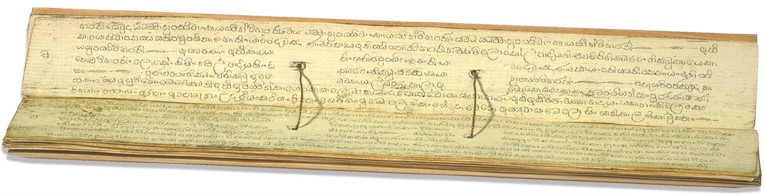
\includegraphics[width=1.0\linewidth]{./Diagrams/Palm}
\caption{These were the kinds of books created during the 4\textsuperscript{th} council and they are still created today.}
\label{fig:Palm}
\end{figure}

Moggaliputta Tissa sent out missionaries after the Third Council and this is how Buddhism was introduced to Sri Lanka at the Mahāvihāra.\footnote{\url{http://en.wikipedia.org/wiki/Anuradhapura_Maha_Viharaya}} For more than 200 years, the Mahāvihāra was the only Buddhist school in Sri Lanka. About 2000 years ago, the Sri Lankan King decided to introduce a new Buddhist school from India, the Abhayagiri\footnote{\url{http://en.wikipedia.org/wiki/Abhayagiri_vihara}} School. The Mahāvihāra now had competition and no longer had royal support. This was one of the factors contributing to the Fourth Council,\footnote{\url{http://en.wikipedia.org/wiki/Fourth_Buddhist_council}} when the Mahāvihāra monks went to a cave away from the royal capital to write their version of the \textit{Tipiṭaka} texts on palm leaves. Once the \textit{Tipiṭaka} had been committed to writing it was more difficult to change, so it is likely that the \textit{Tipiṭaka} that we have today was more or less finalized by the time of the Fourth Council.\footnote{The Fifth Council (\url{http://en.wikipedia.org/wiki/Fifth_Buddhist_council}) and the Sixth Council (\url{http://en.wikipedia.org/wiki/Sixth_Buddhist_council}) were held in Myanmar in 1871 and 1954. They involved a recitation and confirmation of the \textit{Tipiṭaka}.}

Reminds me of a joke: after 2000 years of copying the Buddhist texts, they realized that early on somebody had made a mistake and forgotten the “R”; the original word was “celebrate.”

\subsection*{Buddhaghosa’s Commentaries (compiled about 1500 years ago based on much older material)}

When the Chinese pilgrim monk Faxian\footnote{\url{http://en.wikipedia.org/wiki/Faxian}} visited Sri Lanka in 400 AD, he observed that the Abhayagiri School had 5000 monks, another school closely related to the Abhayagiri School\footnote{The Jetavana School (\url{http://en.wikipedia.org/wiki/Jetavanaramaya}).} had 2000 monks while the Mahāvihāra School had 3000 monks. In other words, 70 percent of the monks in Sri Lanka were not from the Mahāvihāra School. The monks from the Mahāvihāra School were feeling threatened.\footnote{Around 1200 AD the Mahāvihāra gained royal support and were able to eliminate the competing schools.} They were using Pāḷi while their competitors were using Sanskrit. They were seen as conservatives who had nothing new to offer while their competitors were introducing new Mahāyāna practices from India.\footnote{The competition also had a popular meditation manual called the Vimuttimagga, “The Path of Freedom”: (\url{http://en.wikipedia.org/wiki/Vimuttimagga}). Buddhaghosa’s Visuddhimagga was the Theravāda replacement for the Vimuttimagga. The Vimuttimagga and the Visuddhimagga have the same general structure of \textit{Sīla}, \textit{Samādhi} and \textit{Paññā}, but the Vimuttimagga is more practical while the Visuddhimagga is comprehensive and scholarly.} 

Based in the Mahāvihāra, Buddhaghosa\footnote{\url{http://en.wikipedia.org/wiki/Buddhaghosa}} wrote the Visuddhimagga.\footnote{\url{http://en.wikipedia.org/wiki/Visuddhimagga} (Path of Purification, see Footnote 2 for link).} Wikipedia describes the Visuddhimagga as a complete and coherent explanation of the \textit{Tipiṭaka} using the “Abhidhamma method.” Buddhaghosa also compiled Commentaries\footnote{The Visuddhimagga was written first and is referenced in many places in the Commentaries. The Visuddhimagga and the Commentaries provide background stories to the Suttas, word by word analysis of the Suttas, definitions and etymological information for important terms. The Visuddhimagga and the Commentaries are strongly influenced by the Abhidhamma. The Visuddhimagga was written and the Commentaries were compiled about 1000 years after the Buddha’s \textit{parinibbāna} and in a cultural environment that was different from when the Buddha taught. This book is a modern scholar’s attempt to interpret the Buddha’s teachings in their original context: \url{http://www.ahandfulofleaves.org/documents/What the Buddha Thought_Gombrich_2009.pdf}} for most of the texts in the \textit{Tipiṭaka}, based on Sinhalese materials accumulated in the library of the Mahāvihāra.\footnote{Buddhaghosa considered himself to be a compiler and translator of earlier material (not an author) and rarely offered his own views. Everything that he wrote would have been reviewed by the elders of the Mahāvihāra to confirm that it was aligned with the Theravāda doctrine.}

For the Mahāvihāra School, the Commentaries served three purposes. First, they reintroduced Pāḷi as an important language, not a dead language. Second, they presented the Mahāvihāra doctrine and reinforced the importance of the Abhidhamma. Third, they presented all the accumulated traditional accounts to capture the interest of the lay community. Actually, most of the stories about the life of the Buddha taught in Sunday Schools today are not from the Suttas, but are traditional accounts from the Commentaries.\footnote{The Suttas do not contain a lot of biographical material. For details of what is in the Suttas, see \url{http://store.pariyatti.org/Life-of-the-Buddha-The--PDF-eBook_p_1412.html}}

\subsection*{Abhidhammattha Sangaha (about 1000 years ago)}

The Abhidhammattha Sangaha is a very concise summary of the Abhidhamma and its Commentaries written in Sri Lanka about 1000 years ago. The Pāḷi text is only 46 pages long but it summarizes many thousands of pages of material. It was designed for young monks to memorize, without understanding. Once the monks were older, they would study the original Abhidhamma texts using what they had memorized in the Abhidhammattha Sangaha as a foundation. 

\pagebreak

Today, most introductory Abhidhamma courses use the Abhidhammattha Sangaha as their textbook. Twenty years ago, Bhikkhu Bodhi\footnote{\url{http://en.wikipedia.org/wiki/Bhikkhu_Bodhi}} compiled a translation with explanatory notes and charts from Abhidhamma scholars called, “A Comprehensive Manual of Abhidhamma.”\footnote{PDF can be downloaded using the link in Footnote 2. Bhikkhu Bodhi's book is based on Nārada's “A Manual of Abhidhamma” (\url{http://www.buddhanet.net/pdf_file/abhidhamma.pdf}).} With the explanatory notes and charts added, the book is 400 pages long. If, after listening to my Practical Abhidhamma Course, you want to dive deeper into the technical details of the Abhidhamma, I highly recommend this book.\footnote{A three-volume transcript of lectures given by Sayādaw U Sīlānanda using Bhikkhu Bodhi’s book:\\ \url{http://www.abhidhamma.com/Abhid-Lectures-1.pdf}\linebreak \url{http://www.abhidhamma.com/Abhid-Lectures-2.pdf} \linebreak \url{http://www.abhidhamma.com/Abhid-Lectures-3.pdf}\linebreak
YouTube videos of Abhidhamma Retreats (2013 \& 2014) conducted by Bhikkhu Bodhi:\\
\url{https://www.youtube.com/watch?v=kSL1N5caXZM&list=PLgx9_IQQEQyji1DrZK7UDUQp1K7tNIMnW}
\url{https://www.youtube.com/watch?v=GFuVmcXTikw&list=PLgx9_IQQEQyin4DqmOKF4pJxByizw65xT}} Bhikkhu Bodhi’s book is quite technical and detailed. If you are looking for a book that is a bit lighter, I recommend “Abhidhamma in Daily Life” by Nina van Gorkom.\footnote{\url{http://archive.org/details/AbhidhammaInDailyLife}}

\subsection*{Abhidhamma today}

Let’s look at Abhidhamma today. The Abhidhamma is viewed very differently in the three major Theravāda countries: Myanmar,\footnote{\url{http://en.wikipedia.org/wiki/Buddhism_in_Burma}\linebreak\url{http://www.buddhanet.net/pdf_file/bud-myanmar.pdf}} Sri Lanka\footnote{\url{http://en.wikipedia.org/wiki/Buddhism_in_Sri_Lanka}\linebreak\url{http://www.buddhanet.net/pdf_file/bud-srilanka.pdf}} and Thailand.\footnote{\url{http://en.wikipedia.org/wiki/Buddhism_in_Thailand}\linebreak\url{http://www.buddhanet.net/pdf_file/bud-thailand.pdf}}

In Myanmar, Abhidhamma has been studied actively for 900 years.\footnote{“Study of the Abhidhamma amongst the Laity in Myanmar:” \url{http://atbu.org/node/10}} Two hundred fifty years ago, the government was holding exams on Abhidhamma for monks and laypeople.\footnote{The Abhidhamma increased in popularity about 100 years ago when Ledi Sayādaw started promoting \textit{vipassanā} and Abhidhamma for laypeople.} To give you an idea of how popular Abhidhamma is in Myanmar today, in 2005 almost 14,000 laypeople took the basic Abhidhamma exam at 124 government-run centres. Of all of the Theravāda countries, Abhidhamma is most widely studied in Myanmar. Novice monks start studying the Abhidhamma from the age of 13. The Burmese Sayādaws, particularly the meditation teachers, are extremely knowledgeable in Abhidhamma and frequently reference the Abhidhamma during their talks on meditation.

Today in Sri Lanka, the Abhidhamma is studied as an academic topic.\footnote{For example, “The Theravāda Abhidhamma” by Y. Karunadasa and “Abhidhammic Interpretations of Early Buddhist Teachings” by G. D. Sumanapala compare Theravāda Abhidhamma with Abhidharma from other schools.} The Abhidhamma is highly respected in Sri Lanka but rarely mentioned by monks in their Dhamma talks. The late chief monk at the Sri Lankan Vihāra where I teach, Dr. K Sri Dhammananda,\footnote{\url{http://en.wikipedia.org/wiki/K._Sri_Dhammananda}} gave Dhamma talks for 50 years, but I am not aware of him ever talking about Abhidhamma. However, in my early years of teaching,\footnote{I have been teaching Abhidhamma for 15 years at the Buddhist Mahā Vihāra in Kuala Lumpur, Malaysia: \url{http://buddhistmahavihara.org/}} whenever I had a difficult question about Abhidhamma, Chief always had an answer for me.

\pagebreak

In Thailand, the Abhidhamma is generally respected but often not studied in detail as it is in Myanmar.\footnote{The Thais do incorporate the Abhidhamma into a series of funeral chants called the “Abhidhamma \textit{Paṃsukūla}.” This includes 7 brief chants, each chant summarizing one of the books of the Abhidhamma \textit{Piṭaka}. These chants are intended to remind the mourners of the doctrines of \textit{anicca}, \textit{dukkha} and \textit{anattā}.} This is particularly true within the Thai Forest Tradition.\footnote{\url{http://en.wikipedia.org/wiki/Thai_Forest_Tradition}} Many western Theravāda monks are ordained in the Thai Forest Tradition and receive little training in the Abhidhamma. I consider this to be unfortunate, because western audiences are scientifically minded and, to quote a lay Burmese Abhidhamma teacher, “Abhidhamma is the Ultimate Science.”\footnote{The title of Dr. Mehm Tin Mon’s translation of the Abhidhammattha Sangaha with Commentary: \url{http://www.buddhanet.net/pdf_file/abhidhaultsci.pdf}} I believe that, if properly presented, Abhidhamma would be extremely popular in the West because it is so scientific, and can be applied both to daily life and to meditation practice.

\subsection*{Linkage to \textit{Satipaṭṭhāna} Sutta}
Now let’s relate this historical material to the \textit{Satipaṭṭhāna} Sutta.\footnote{For an analysis of the \textit{Satipaṭṭhāna} Sutta see \url{http://santifm.org/santipada/wp-content/uploads/2012/08/A_History_of_Mindfulness_Bhikkhu_Sujato.pdf} and \url{http://www.buddhismuskunde.uni-hamburg.de/pdf/5-personen/analayo/direct-path.pdf}}

There are two versions of the \textit{Satipaṭṭhāna} Sutta in the Sutta \textit{Piṭaka}; the version in the Appendix is from the \textit{Majjhima Nikāya}, and there is another version in the \textit{Dīgha Nikāya}.\footnote{DN 22: \url{http://www.accesstoinsight.org/tipitaka/dn/dn.22.0.than.html}} The two versions are virtually identical, except that the version in the \textit{Dīgha Nikāya} adds a long explanation of the Four Noble Truths. 

If the Commentaries are correct and all the Suttas were actually finalized at the First Council, we should ask ourselves, “Which version did the Buddha actually teach on that day?”

When Xuanzang returned to China, he took back two versions of the \textit{Satipaṭṭhāna} Sutta from non-Theravāda Buddhist schools. The Theravāda version and the two Chinese versions are quite similar so it is clear they came from a common source that existed before the split of the Sangha.\footnote{For details, see “A Comparative Study of the Majjhima Nikāya,” Volume 1, pages 73--97.} One difference is that the Chinese versions do not include the aggregates or the Four Noble Truths. If the version of the \textit{Satipaṭṭhāna} Sutta that existed before the split of the Sangha did include the aggregates and the Four Noble Truths, it is unlikely they would have been deleted by the other schools because these are core teachings. 

Therefore, I believe that the aggregates and Four Noble Truths were added to the Theravāda version of the \textit{Satipaṭṭhāna} Sutta sometime after the split of the Sangha. The aggregates and Four Noble Truths are core teachings of the Buddha, but I believe that their incorporation into the \textit{Satipaṭṭhāna} Sutta was a later addition.

I have picked one part of the \textit{Satipaṭṭhāna} Sutta to illustrate this point, but evidence of additions, editing and rearrangement, can be found in many other Suttas as well. In my opinion, the Suttas were not finalized at the First Council; the Suttas evolved over time. My conclusion is that the Theravāda Suttas we have today contain the teachings of the Buddha, but they are \textbf{not} the literal, verbatim “word of the Buddha.” Personally, I am not disturbed by this because to me, it is the \textbf{teachings} that are important; the words merely point to the teachings.

\pagebreak

\begin{figure}[H]
\begin{tabular*}{\textwidth}{L{\dimexpr0.5\textwidth-2\tabcolsep} | L{\dimexpr0.5\textwidth-2\tabcolsep}}
\toprule
\tableheader{Structure of the Satipaṭṭhāna Sutta\newline from the Abhidhamma Piṭaka} & \tableheader{Structure of the Satipaṭṭhāna Sutta\newline from the Majjhima Nikāya} \\
\midrule
\textbf{The Contemplation of the Body} & \textbf{The Contemplation of the Body} \\
& Mindfulness of Breathing \\
& Postures of the Body \\
& Mindfulness with Clear Comprehension \\
Reflection on the Repulsiveness of the Body & Reflection on the Repulsiveness of the Body \\
& Reflection on the Material Elements \\
& Nine Cemetery Contemplations\\
& \\
\textbf{The Contemplation of Feeling} & \textbf{The Contemplation of Feeling} \\
Types of Feeling & Types of Feeling \\
& \\
\textbf{The Contemplation of Consciousness} & \textbf{The Contemplation of Consciousness} \\
Types of Consciousness & Types of Consciousness \\
& \\
\textbf{The Contemplation of Mental Objects} & \textbf{The Contemplation of Mental Objects} \\
Five Hindrances & Five Hindrances \\
& Five Aggregates of Clinging \\
& Six Internal and Six External Sense Bases \\
Seven Factors of Enlightenment & Seven Factors of Enlightenment \\
& Four Noble Truths\\

\bottomrule

\end{tabular*}
\caption{Comparing the Satipaṭṭhāna Sutta from the Abhidhamma Piṭaka (Vibhaṅga) and the Satipaṭṭhāna Sutta from the Majjhima Nikāya suggests that the Abhidhamma version may be earlier and that additions may have been made (from other Suttas) to the Majjhima Nikāya version.}
\label{fig:Satipatthana}
\end{figure}

We do not even have to look at other Buddhist schools to find inconsistency in the \textit{Satipaṭṭhāna} Sutta. One of the seven books of the Abhidhamma\footnote{“The Book of Analysis” (\textit{Vibhaṅga}), pages 251--270.} includes an essay that analyzes \textit{Satipaṭṭhāna} from both the Sutta perspective, and from an Abhidhamma perspective. The Abhidhamma text quotes the complete \textit{Satipaṭṭhāna} Sutta. This version of the Sutta does not include the aggregates or Four Noble Truths under the Contemplation of Mental Objects.

There is an even bigger inconsistency when looking at the Contemplation of the Body. The \textit{Satipaṭṭhāna} Sutta from the \textit{Majjhima Nikāya} includes \textbf{Mindfulness} of breathing, postures of the body, mindfulness with clear comprehension, reflection on the repulsiveness of the body, reflection on the material elements and nine cemetery contemplations. The \textit{Satipaṭṭhāna} Sutta from the Abhidhamma includes only reflection on the repulsiveness of the body. 

My conclusion is that from the time that this portion of the Abhidhamma was finalized, and the time that the \textit{Satipaṭṭhāna} Sutta from the \textit{Majjhima Nikāya} was finalized, sections were added to include \textbf{Mindfulness} of breathing, postures of the body, \textbf{Mindfulness} with clear comprehension, reflection on the material elements and nine cemetery contemplations. In other words, I believe that the Abhidhamma and the Suttas were evolving in parallel.

\pagebreak

\subsection*{Summary of Key Points}

\begin{itemize}

\item Buddhist teachings come from four periods: the Suttas and Vinaya, the Abhidhamma, the Commentaries and from modern teachers. The teachings of each period build on teachings of the previous periods. To provide context, it is useful to know the period from which a teaching comes.

\item According to the traditional account from the Commentaries, the Buddha first taught the Abhidhamma in one of the heavens and then passed a summary to Sāriputta, who compiled the Abhidhamma texts that we have today (except for one book which was authored about 250 years later).

\item According to scholars, about 100 years after the Buddha’s \textit{parinibbāna}, when the Sangha split, the main Buddhist doctrines were already fixed, though the Suttas were still subject to editing. At this time, the organization of Suttas into \textit{Nikāyas} was in progress and the Abhidhamma had not been formalized.

\begin{itemize}

\item In my opinion, the Abhidhamma is not the “word of the Buddha,” but I also believe that the Suttas are not the  literal, verbatim “word of the Buddha;” in my opinion, the Abhidhamma was evolving while the Suttas were being finalized and this can be seen by comparing the version of the \textit{Satipaṭṭhāna} Sutta found in the Abhidhamma with the version found in the \textit{Nikāyas}.

\end{itemize}

\item Factors that contributed to the development of the Abhidhamma may include:

\begin{itemize}

\item The need for a systematized structure covering all Suttas to resolve questions and to instruct novice monks.

\item A reaction to the trend among contemporary “atomist” philosophers to identify “irreducible components” or Ultimate Realities.

\item The need to organize the content of the Suttas in a way that emphasized the unique doctrines of the Theravāda school.

\end{itemize}

\item Buddhaghosa’s Visuddhimagga and the Commentaries make extensive use of the Abhidhamma; they were written in the fifth century.

\item The Abhidhammattha Sangaha is a summary of the Abhidhamma and Commentaries, intended for novice monks to memorize; it was written in the tenth century.

\item Today, the Abhidhamma is highly esteemed in Myanmar, often treated as an academic subject in Sri Lanka and often not studied in detail in Thailand.

\end{itemize}

Finally, in my opinion, the most important thing to remember about this lesson is that there are four sources of teachings: Suttas, Abhidhamma, Commentaries and modern teachers. Each builds on the earlier sources. Each of these sources are useful and knowing the source of a specific teaching helps to provide context.

\newpage

\subsection*{Questions \& Answers}

\question{Where does “The Questions of King Milinda” fit into this timeline?}

\begin{figure}[H]
\begin{quoting}
\topsep=0pt
\begin{flushleft}
\vspace{-1mm}
\textit{By what name shall I know you, Sir?}
\vspace{-1mm}
\end{flushleft}
\begin{flushright}
\vspace{-1mm}
\textit{My companions call me Nāgasena. But the name and the\linebreak person to whom the name refers do not really exist.}
\vspace{-1mm}
\end{flushright}
\begin{flushleft}
\vspace{-1mm}
\textit{If Nāgasena and the person do not exist, to whom do\linebreak people offer alms and who receives these offerings?\linebreak Since you receive them, you really exist.}
\vspace{-1mm}
\end{flushleft}
\begin{flushright}
\vspace{-1mm}
\textit{Your Majesty, did you come to this\linebreak monastery on foot or by chariot?}
\vspace{-1mm}
\end{flushright}
\begin{flushleft}
\vspace{-1mm}
\textit{I came by chariot.}
\vspace{-1mm}
\end{flushleft}
\begin{flushright}
\vspace{-1mm}
\textit{Well then, what is a chariot? Is the horse the chariot?\linebreak Is the wheel the chariot? Is the axle the chariot?\linebreak Is the carriage the chariot?}
\vspace{-1mm}
\end{flushright}
\begin{flushleft}
\vspace{-1mm}
\textit{I must answer “No” to all of your questions.}
\vspace{-1mm}
\end{flushleft}
\begin{flushright}
\vspace{-1mm}
\textit{Is there a thing called chariot beside the horse,\linebreak the wheel, the axle, the carriage, etc.?}
\vspace{-1mm}
\end{flushright}
\begin{flushleft}
\vspace{-1mm}
\textit{There is no chariot beside the horse, the wheels,\linebreak the axle and the carriage. Just a combination of\linebreak these things has been named a chariot.}
\vspace{-1mm}
\end{flushleft}
\begin{flushright}
\vspace{-1mm}
\textit{Very well, your Majesty, you should understand\linebreak Nāgasena as you understood the chariot.}
\vspace{-1mm}
\end{flushright}
\end{quoting}

\caption{King Milinda meets Nāgasena; the “components of the chariot” are the five aggregates (see also \url{http://www.accesstoinsight.org/tipitaka/sn/sn05/sn05.010.bodh.html}). }
\label{fig:Milinda}
\end{figure}

“The Questions of King Milinda” was written about 2100 years ago.\footnote{See \url{http://www.aimwell.org/milinda.html} and \url{http://en.wikipedia.org/wiki/Milinda_Panha}} It is included in the Burmese \textit{Tipiṭaka} but not in the Thai or Sri Lankan \textit{Tipiṭaka}.

It is written in the form of a dialogue between King Milinda and a Buddhist Monk, Nāgasena. King Milinda was an actual historical figure, a Greek king who ruled the kingdom of Bactria.\footnote{The Greek kingdom of Bactria (\url{http://en.wikipedia.org/wiki/Bactria}), in modern-day Afghanistan, was established by Alexander the Great. King Milinda (Greek name: Menander I, (\url{http://en.wikipedia.org/wiki/Menander_I}) ) extended the kingdom into North India and converted to Buddhism. Milinda and his successors were supporters of Buddhism. The first representations of the Buddha as a human date from this period and even today, paintings and statues of the Buddha show a Greek influence (\url{http://en.wikipedia.org/wiki/Greco-Buddhist_art}). Interestingly, the Suttas clearly state that the Buddha was bald, but even today all representations of the Buddha show him with a full head of hair! For the first 500 years, the Buddha was represented by an icon such as a stupa, footprint, bodhi tree, or wheel rather than as a human.} In a typical exchange, King Milinda would ask a philosophical question\footnote{The questions posed by King Milinda demonstrate a knowledge of the Suttas and show an influence of the Upaniṣads rather than an influence of Greek philosophy.} and Nāgasena would then give a reply using an analogy to explain his point clearly. 

\question{According to the traditional account, the Abhidhamma came before the Suttas and the Vinaya, so why isn't the Abhidhamma the first \textit{Piṭaka}?}

The \textit{Tipiṭaka} is not organized chronologically. For example, the first Sutta delivered by the Buddha, the Dhammacakkappavattana Sutta (SN 56.11: \url{http://www.accesstoinsight.org/tipitaka/sn/sn56/sn56.011.harv.html}) is located near the end of the third \textit{Nikāya}.

\question{Are you suggesting that we prioritize teachings based on the historical period in which they originate?}

Some modern teachers such as Mahāsi Sayādaw and Ajahn Chah add significant value to what had been taught previously in the Suttas, Abhidhamma and Commentaries. However, a few modern teachers misrepresent the earlier teachings (either unintentionally due to ignorance or intentionally due to arrogance).

Not everything presented in Dhamma talks or in Dhamma books comes from the Suttas. Forming a habit of asking oneself, “what is the original source for this idea?” does not mean to be critical or analytical;\footnote{Trying to identify the specific Sutta or source text is being analytical and can be a distraction.} it simply means to be aware of the context of a teaching. Remember that one of the qualities of the Dhamma is \textit{ehipassiko}, which means “inviting inspection.” 

\question{You mentioned that different schools have different versions of Abhidhamma. How do we know that we are studying the right one?}

In my opinion, we should not think in terms of “right” or “wrong,” but rather, how useful the Abhidhamma is in deepening our understanding of the Suttas and in supporting our practice. If history had worked out a bit differently, we might be studying one of the other versions of Abhidhamma today, but as it is, we have the Theravāda version as a living tradition with many resources available. In my opinion, we should focus on the practical aspects rather than on a scholarly perspective.

\question{Mindfulness Based Stress Reduction (MBSR) is becoming popular. Can the Abhidhamma be applied to MBSR?}

Mindfulness Based Stress Reduction\footnote{\url{http://en.wikipedia.org/wiki/Mindfulness-based_stress_reduction}} was developed 25 years ago by an American mental health professional.\footnote{Dr. Jon Kabat-Zinn: \url{http://en.wikipedia.org/wiki/Jon_Kabat-Zinn}} The MBSR program\footnote{Described in \url{http://www.amazon.com/Full-Catastrophe-Living-Wisdom-Illness/dp/0739358588}} is a pure mindfulness exercise, similar in some ways to basic \textit{vipassanā} meditation practice, but without spiritual content (as the name suggests, MBSR is for stress reduction). Even though MBSR does not lead to spiritual development, according to WebMD, depression affects almost one in six people at some point in their lives,\footnote{\url{http://www.webmd.com/depression/ss/slideshow-depression-myths}} so the secular practice of MBSR can help our society. 

In my opinion, for the mental health industry to take MBSR to the next level, they will need a framework and standardized, specialized terminology to structure their discussions and analyze the mind in more detail. I believe that many aspects of the Abhidhamma can be repurposed to a secular context to accelerate this progress.

\pagebreak

\question{What is the relationship between the Visuddhimagga and the Commentaries?}

Buddhaghosa wrote the Visuddhimagga and was the compiler/translator of the Commentaries.

According to legend,\footnote{Chapter XXXVII of the Cūḷavamsa, written 800 years after Buddhaghosa died.} Buddhaghosa was born near Bodh Gaya\footnote{\url{http://en.wikipedia.org/wiki/Bodh_Gaya}} to a Brahmin\footnote{\url{http://en.wikipedia.org/wiki/Brahmin}} family. In the Indian caste system, Brahmins were priests who memorized and recited the \textit{Vedas}.\footnote{\url{http://en.wikipedia.org/wiki/Vedas}} As a young man, Buddhaghosa established himself as a famous debater. A Buddhist monk, Revata, decided to convert Buddhaghosa to Buddhism. One day while Buddhaghosa was reciting the \textit{Vedas}, Revata called out, “Who is this man, braying like a donkey?” Buddhaghosa replied, “So, you think that you understand the language of a donkey?” and the debate started! Revata proved that he understood the \textit{Vedas} and pointed out areas where they were wrong. Defeated, Buddhaghosa asked, “So what is your doctrine?” Revata then quoted from the Abhidhamma and Buddhaghosa could not respond. He was deeply impressed by the Abhidhamma. He was converted to Buddhism and that is when he got the name Buddhaghosa. \textit{Ghosa} is Pāḷi for “voice” so the name Buddhaghosa literally means “voice of the Buddha.”

Revata told Buddhaghosa to go to the Mahāvihāra in Sri Lanka to compile the commentaries that had been collected in Sinhalese and translate them into Pāḷi. Buddhaghosa went to the Mahāvihāra and said to the temple elders, “Please open up your library to me.” The elders replied, “To show that you are worthy, write an essay on the topic of virtue, concentration and understanding.” So Buddhaghosa composed the Visuddhimagga, an 800-page treatise detailing the Theravāda doctrine that draws heavily on the Abhidhamma.

After Buddhaghosa wrote the Visuddhimagga, the gods made the book disappear, so he had to write it down again. Again the gods made this version disappear, so he wrote the book a third time. Then the gods allowed the previous two versions to be visible and the elders were amazed that all three versions were absolutely identical. A later legend says that Buddhaghosa wrote the Visuddhimagga out three times in one night. 

The elders were impressed by the Visuddhimagga and allowed Buddhaghosa access to the library. He compiled commentaries on most of the Vinaya, Suttas and Abhidhamma. For the commentaries, Buddhaghosa saw himself as a compiler/translator of much older materials, some of which may have originated at the time of the Buddha 1000 years earlier.

Whereas the Visuddhimagga focuses on explaining Theravāda doctrine, the Commentaries focus on explaining the Vinaya, Suttas and Abhidhamma. The Commentaries include a lot of stories such as the background leading up to a Sutta being delivered. They also discuss grammatical points and word derivations to make sure that the Vinaya, Suttas and Abhidhamma are clearly understood. When it comes to doctrinal points, the Commentaries often reference the Visuddhimagga; this shows that the Visuddhimagga was written before the Commentaries. 

Though Buddhaghosa prepared Commentaries for most of the \textit{Tipiṭaka}, the Commentaries for some portions of the \textit{Tipiṭaka} were complied later by other authors. In addition, sub-commentaries were written for many of the Commentaries to provide even more detailed explanations.

\pagebreak

\question{What are the main differences between the Abhidhammattha Sangaha and the original seven Abhidhamma texts?}

The Abhidhammattha Sangaha is a concise summary written almost 1500 years after the original seven Abhidhamma texts. The main topics of the Abhidhammattha Sangaha are:

\begin{itemize}

\item Mind Moments: Both the Abhidhammattha Sangaha and the original text (\textit{Dhammasaṅgaṇī}) include 89 Mind Moments, though the sequence of presentation is slightly different.

\item Mental Factors: The Abhidhammattha Sangaha has a fixed list of 52 Mental Factors. The original text (\textit{Dhammasaṅgaṇī}) has open-ended lists that include many overlapping terms but do not mention Mental Factors such as \textbf{Attention}, \textbf{Determination}, \textbf{Motivation}, \textbf{Compassion}, \textbf{Sympathetic joy} and the three abstinences.

\item \textit{Rūpa}: The Abhidhammattha Sangaha has a fixed list of 28 \textit{rūpa} and discusses groups of \textit{rūpa} (\textit{kalāpa}). The original text (\textit{Dhammasaṅgaṇī}) has a fixed list of 27 \textit{rūpa} (not including \textbf{Heart-base}) and does not discuss groups of \textit{rūpa}.

\item Realms of Existence: Both the Abhidhammattha Sangaha and the original texts have the same list of realms of existence. The Abhidhammattha Sangaha gives a detailed analysis of Mind Moments leading to rebirth in specific realms. The original text (\textit{Vibhaṅga}) just mentions the lifespan in each realm.

\item Processes: The Abhidhammattha Sangaha has a detailed description of sense-door processes, mind-door processes, jhāna processes and rebirth processes. The original text (\textit{Paṭṭhāna}) hints at processes and the Commentaries have a very general description of only the sense-door process.

\item Conditions: The Abhidhammattha Sangaha has a very concise summary of the 24 conditions and introduces sub-categories under some conditions (for example, natural decisive support is introduced as a sub-category under decisive support condition). The original text (\textit{Paṭṭhāna}) has a very detailed description of the 24 conditions.

\item Meditation Subjects: The Abhidhammattha Sangaha describes the meditation subjects for both \textit{samatha} and \textit{vipassanā}. The original texts do not touch on this subject; it is discussed in some detail in the Visuddhimagga.

\end{itemize}
